\section{Exercise 2}
\begin{enumerate}[label=\arabic*.]
    \item $a_{11} = a_{22} = a_{33} =0 $, how many of the six terms in
        $\text{det} A$ will be zero? If $a_{11} = a_{22} = a_{33} = a_{44}
        = 0 $, how many of the 24 products $a_{1j}a_{2k}a_{3l}a_{4m}$ are
        zero?
        \begin{mdframed}[style=MyFrame]
            Starting with the determinant formula for a $3 \times 3$
            matrix, namely
            \begin{equation}
                \text{det}A =
                    a_{11}(a_{22}a_{33} - a_{23}a_{32})
                    -a_{12}(a_{21} a_{33} - a_{23}a_{31})
                    + a_{13}(a_{21}a_{32} -a_{22}a_{31})
            \end{equation}
            Multiply everything out gives,
            \begin{equation}
                \text{det}A = 
                    a_{11}a_{22}a_{33} 
                    -a_{11}a_{22}a_{23}  
                    -a_{12}a_{21}a_{33}  
                    +a_{12}a_{23}a_{31}  
                    +a_{13}a_{21}a_{32}  
                    -a_{13}a_{22}a_{31}  
            \end{equation}
            Substituting in $a_{11} = a_{22} = a_{33} =0 $ we get,
            \begin{equation}
                \text{det}A = 
                    -a_{12}a_{23}a_{32} + a_{13}a_{21}a_{31}
            \end{equation}
            Thus we see that 4 out of the 6 terms are zero. Furthermore the
            same analysis can be done to show that there are 15 zero terms
            in for the second part of the question. 
        \end{mdframed}


                
    \item Show that 4 is the largest determinant for a $3 \times 3$ matrix
        of $1's$ and $-1's$.
        \begin{mdframed}[style=MyFrame]
            In order to show that the largest determinant is 4 a simple
            python code was written to test all 512 permutations of the
            matrix. Figure~(\ref{fig:det}) clearly shows that the largest
            determinant that can be produced for the matrix described is 4.
            \begin{figure}[H]
                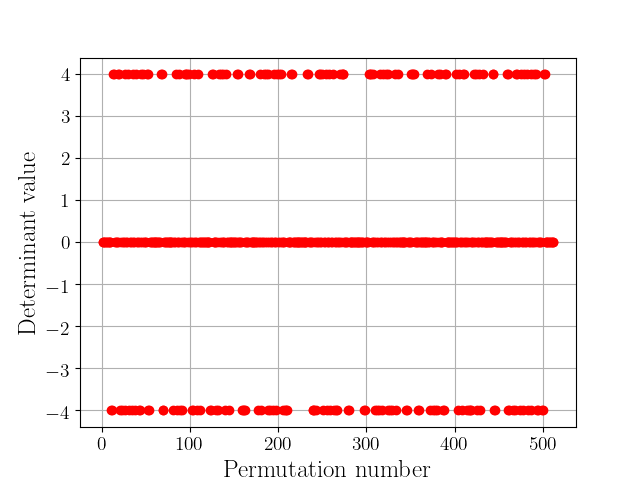
\includegraphics[height=0.35\textheight]{../media/determinant-study.png}
                \caption{Determinant study for a matrix of $\pm 1$}
                \label{fig:det}
            \end{figure}
            \emph{\textbf{See Appendix for attached code}}
        \end{mdframed}

    \item Find the cofactors and put them into cofactors matrices $C$ and
        $D$. Find $AC$ and $\text{det}B$.
        \begin{equation}
          A = 
          \begin{bmatrix}
            a & b \\
            c & d
           \end{bmatrix}
        \end{equation}
        and 
        \begin{equation}
            B = 
            \begin{bmatrix}
                1 & 2 & 3 \\
                4 & 5 & 6 \\
                7 & 0 & 0
            \end{bmatrix}
        \end{equation}

    \item Find the cofactors matrix $C$ and multiply $A$ times $C^{T}$.
        Compare $AC^{T}$ with $A^{-1}$:
        \begin{equation}
            A =
            \begin{bmatrix}
                2 & -1 & 0 \\
                -1 & 2 & -1 \\
                0 & -1 & 2
             \end{bmatrix}
        \end{equation}
\end{enumerate}
